\documentclass[../../main.tex]{subfiles}
\begin{document}
\chapter{Rigging and Layers}
\label{ch:rigging_layers}

\section{Introduction}
In computer graphics, rigging involves setting up a skeletal structure (also known as an armature) that drives the mesh of a character, allowing it to move and deform in a realistic manner. Rigging is a critical component of character animation, as it determines how the character responds to movement and how it deforms during animation. In the context of sign language avatars, rigging plays a crucial role in capturing the complex articulations and expressions of sign language gestures.

The layered approach to rigging, which this chapter explores in depth, offers a sophisticated method for managing these complexities. By dividing the rigging process into several distinct layers—each responsible for a different aspect of the avatar’s movement and deformation—we can achieve a higher level of control and flexibility. This approach not only facilitates the creation of more natural and expressive animations but also makes the system scalable and adaptable to a wide range of linguistic contexts.

In this chapter, we will delve into the theoretical foundations of layered rigging, review related work, describe the specific layers used in our system, and discuss the results and implications of this approach. We will also outline future directions for improving the integration of procedural methods with traditional animation techniques.

\section{Procedural Rigging for Signing Avatars}

Rigs have been used in computer animation for decades to control the movement and deformation of characters. Traditional rigging systems typically consist of a hierarchical structure of bones, controllers, and constraints that define how the character’s mesh deforms in response to movement. Section {subsubsec:skeleton} in chapter {ch:background_work} gave an overview of the different skeletal structures of an avatar and how it is used to control the character’s movements.

A signing avatar differs significantly from the traditional systems. For starter, no sign language uses the lower body in its articulation. This means that the rigging system for a signing avatar can be simplified to focus on the upper body as shown in figure \ref{ref:upper_body_avatar}. 

\begin{figure}[h]
    \centering
    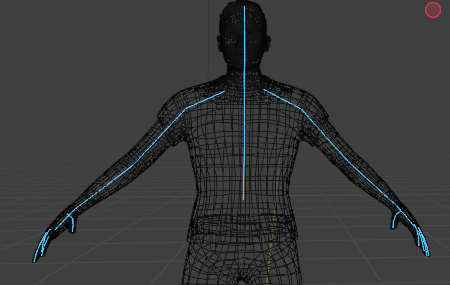
\includegraphics[width=0.5\textwidth]{chapters/rigging_layers/images/upper_body_avatar.png}
    \caption{An example of an upper body avatar rig}
    \label{ref:upper_body_avatar}
\end{figure}

However for procedurally animating a signing avatar, the complexity of sign language gestures and expressions poses unique challenges and necessitates a more sophisticated rigging system.

\subsection{AZee Blender interface}

The previous low level synthesizor for AZee \cite{fabrizio} used an armature in blender with todo bones and todo sites. These bones and sites were mapped to a \emph{SkelSpec} structure. Similarly, AZee's abstract posture was mapped to the \emph{SkelSpec} structure as well. The \emph{SkelSpec} structure thus formed as an intermediate bridge between an Animated AZee Score and the armature \ref{fig:old_interface}. 

\begin{figure}[h]
    \centering
    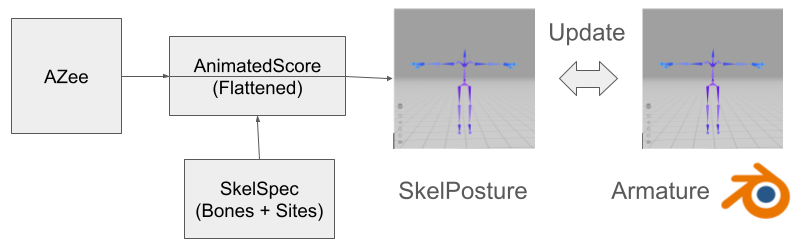
\includegraphics[width=0.5\textwidth]{chapters/rigging_layers/images/old_interface.png}
    \caption{The old interface of the low level synthesizor for AZee}
    \label{fig:old_interface}
\end{figure}

One of the first contributions of my work was to create a new interface for the low level synthesizor for AZee. This new interface didn't have a \emph{SkelSpec} \ref{fig:new_interface} and interacted directly with the blender armature resulting in faster executions \ref{tab:faster_executions}.

\begin{figure}[h]
    \centering
    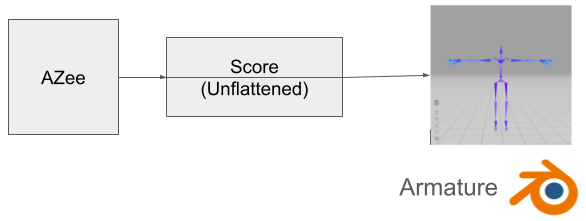
\includegraphics[width=0.5\textwidth]{chapters/rigging_layers/images/new_interface.png}
    \caption{The new interface of the low level synthesizor for AZee}
    \label{fig:new_interface}
\end{figure}

\begin{table}
    \centering
    \begin{tabular}{|c|c|}
        \hline
        \textbf{Interface} & \textbf{Execution time (s)} \\
        \hline
        Old & 0.5 \\
        New & 0.2 \\
        \hline
    \end{tabular}
    \caption{Comparison of execution times between the old and new interfaces}
    \label{tab:faster_executions}
\end{table}

\subsection{Automatic site generation}

The previous low level synthesizor for AZee \cite{fabrizio} required the user to manually create sites in blender. This was a tedious time consuming process process and could lead to errors \ref{fig:prev_sites}.

\begin{figure}[h]
    \centering
    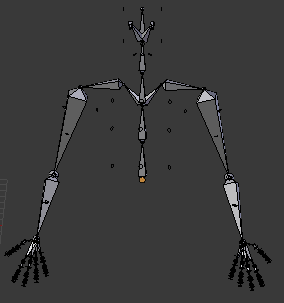
\includegraphics[width=0.5\textwidth]{chapters/rigging_layers/images/prev_sites.png}
    \caption{Manually created sites in the previous low level synthesizor for AZee}
    \label{fig:prev_sites}
\end{figure}

This site generation process could be partially automated if we have the knowledge of the bone structure. Algorithm was used to generate sites based on bone location and avatar mesh using simple raycasting \ref{alg:raycasting}.

TODO
\begin{algorithm}
    \label{alg:raycasting}
    \caption{Raycasting algorithm for automatic site generation}
    \begin{algorithmic}
        \State $bones \gets$ get all bones in the armature
        \For{$bone$ in $bones$}
            \State $head \gets$ get the head of the bone
            \State $tail \gets$ get the tail of the bone
            \State $midpoint \gets$ get the midpoint of the bone
            \State $direction \gets$ get the direction of the bone
            \State $site \gets$ create a site at the midpoint of the bone
            \State $site \gets$ move the site in the direction of the bone
        \EndFor
    \end{algorithmic}
\end{algorithm}

\subsection{Constraint Optimization}

The previous low level synthesizor for AZee \cite{fabrizio} used a constraint optimization algorithm to generate the armature pose. This algorithm \ref{alg:old_constraint_optimization} TODO


\begin{algorithm}
    \label{alg:old_constraint_optimization}
    \caption{Old constraint optimization algorithm}
    \begin{algorithmic}
        \State $constraints \gets$ get all constraints in the armature
        \For{$constraint$ in $constraints$}
            \State $constraint \gets$ apply the constraint to the armature
        \EndFor
    \end{algorithmic}
\end{algorithm}



\subsection{Procedural Animation Methods}
To address the limitations of pre-recorded animation techniques, researchers have explored procedural methods for sign language synthesis. Procedural animation involves generating motion dynamically based on a set of rules or constraints, rather than relying on pre-existing data. This approach offers greater flexibility and scalability, as it can generate novel animations on-the-fly, tailored to specific linguistic or contextual needs.

The AZee model (Filhol et al., 2014) represents a significant advancement in this area. AZee allows for the parameterization of sign language gestures based on semantic functions, enabling the synthesis of complex utterances with precise control over timing, concurrency, and non-manual features. By generating a timeline that specifies every aspect of the utterance, AZee overcomes many of the synchronization issues inherent in earlier models.

Despite these advancements, procedural methods face challenges in achieving the same level of naturalness and expressivity as pre-recorded animations. This has led to the development of hybrid approaches that combine the strengths of both techniques, as well as the exploration of more sophisticated rigging systems, such as the layered approach described in this chapter.

\section{Procedural Rigging}
Procedural rigging refers to the process of generating the rig (skeletal structure) of a character dynamically, based on procedural rules or constraints. In the context of sign language avatars, procedural rigging allows for the creation of rigs that can adapt to different gestures, expressions, and movements in real-time, without the need for extensive manual setup.

\subsection{Site Objects}
TODO: Elaborate on the concept of site objects in procedural rigging and their role in facilitating dynamic adjustments to the rig based on linguistic input.

\section{Layers in Avatars}
The layered approach to rigging involves dividing the rigging process into several distinct layers, each responsible for different aspects of the avatar's movement and deformation. This modular approach allows for greater flexibility and control, enabling animators to fine-tune each layer independently while maintaining overall coherence in the final animation.

\subsection{Deformation Bone Layer}
The deformation bone layer is the foundation of the avatar's rig. It includes the bones that directly influence the mesh of the character, controlling how the skin deforms in response to movement. This layer is responsible for the overall shape and posture of the avatar, ensuring that the character's movements are smooth and realistic.

In this layer, the bones are typically organized into a hierarchy, with the root bone controlling the overall position and orientation of the avatar, and child bones controlling specific parts of the body, such as the limbs, spine, and head. Weight painting is used to determine how much influence each bone has over the surrounding mesh, allowing for precise control over how the character's skin deforms.

One of the key challenges in the deformation bone layer is managing the interaction between different parts of the body. For example, when the arm moves, the shoulder and spine must also adjust to maintain a natural posture. This requires careful consideration of joint constraints and the use of advanced techniques such as dual quaternion skinning to prevent artifacts such as "twisting" or "collapsing" of the mesh.

\subsection{Inverse Kinematics Layer}
The inverse kinematics (IK) layer is responsible for positioning the avatar's limbs by solving for the joint angles required to achieve a desired end-effector position. In the context of sign language avatars, this is particularly important for ensuring that the hands can accurately perform the required gestures.

IK is a powerful tool for animators because it allows them to specify the position of the end of a limb (such as a hand or foot) and have the software automatically calculate the necessary joint rotations to achieve that position. This is particularly useful for tasks that require precise control over the hands, such as signing, where the exact position and orientation of the hands are critical.

However, IK also presents certain challenges. One issue is that the solution provided by the IK solver may not always be physically plausible or aesthetically pleasing. For example, an IK solution might place the hand in the correct position but result in unnatural rotations of the elbow or shoulder. To address this, additional constraints are often applied to limit the range of motion of the joints and to prioritize certain joints over others.

In our layered approach, the IK layer is closely integrated with the deformation bone layer, ensuring that the movements generated by the IK solver are consistent with the overall posture of the avatar. This integration is achieved through the use of custom IK solvers and constraints that take into account the specific requirements of sign language gestures.

\subsection{Forward Kinematics Layer}
The forward kinematics (FK) layer controls the rotation of bones in a hierarchical manner, where the rotation of a parent bone affects all its children. This layer is used for broader, more deliberate movements, such as head tilts, body leans, or full-body rotations, which are important for conveying non-manual signals in sign language.

FK provides animators with a high degree of control over each individual bone in the rig, allowing for precise adjustments to the character's pose. Unlike IK, where the position of the end-effector is specified, FK requires the animator to manually rotate each bone in the chain, starting from the root and working down to the extremities. This can be more time-consuming but offers greater flexibility in achieving complex poses.

In the context of sign language avatars, the FK layer is particularly important for managing non-manual signals, which often involve subtle movements of the head, eyes, and torso. By combining FK with IK, animators can create complex, coordinated movements that integrate both deliberate and reactive motions.

\subsection{Morphs}
Morphs are predefined shape keys that alter the mesh of the avatar independently of the skeletal structure. They are used to control finer details of the avatar's appearance, such as facial expressions, muscle bulges, or specific gestures that cannot be easily achieved through bone manipulation alone.

In sign language avatars, morphs play a crucial role in conveying the subtleties of facial expressions, which are an integral part of the language. For example, raising the eyebrows, furrowing the brow, or tightening the lips can all significantly change the meaning of a sign. Morphs allow these expressions to be blended smoothly with the skeletal movements, ensuring that the avatar's face remains expressive and natural throughout the animation.

Morph targets are typically created by sculpting the mesh into different shapes and then saving these shapes as "keys." During animation, these keys can be blended together in various combinations to achieve the desired expression. The morph layer interacts with the other layers by adjusting the mesh deformation in response to the skeletal movement, ensuring that the overall appearance of the avatar remains cohesive.

\section{Methodology}
This section details the methodology used to implement the layered rigging system in our sign language avatar synthesis model. The approach combines procedural techniques with traditional animation workflows, implemented within Blender, to create a flexible and scalable system for generating realistic sign language animations.

\subsection{Layer Integration}
TODO: Discuss how the different layers (Deformation Bone, IK, FK, Morphs) are integrated into a cohesive system. Explain the process of blending between layers and managing dependencies between them.

\subsection{AZee Model Implementation}
The AZee model serves as the linguistic foundation for our sign language synthesis system. This model allows for the parameterization of sign language gestures based on semantic functions, which are then mapped to specific constraints and actions within the rigging system.

The implementation of AZee within our layered rigging system involves translating the linguistic descriptions into a sequence of constraints that are applied to the appropriate layers. For example, a description might specify the position of the hands, the orientation of the head, and the configuration of the fingers, all of which are handled by different layers within the rig.

The AZee model also provides a framework for managing the timing and concurrency of gestures, ensuring that the various components of a sign are synchronized correctly. This is particularly important for complex utterances that involve multiple simultaneous actions, such as pointing while raising the eyebrows or tilting the head.

\subsection{Data-Driven Synthesis}
In addition to procedural methods, our system incorporates data-driven synthesis techniques to enhance the realism and naturalness of the animations. Pre-recorded motion data is used to inform the procedural generation of movements, providing a reference for achieving lifelike gestures.

Data-driven synthesis is particularly useful for capturing the nuances of sign language that are difficult to model procedurally, such as the fluidity of hand movements or the subtle changes in posture that occur during signing. By combining these techniques with the AZee model, we can generate animations that are both accurate and expressive.

\subsection{Implementation in Blender}
Blender, a popular open-source 3D creation suite, was chosen as the platform for implementing our layered rigging system. Blender's flexible rigging tools and support for Python scripting made it an ideal choice for developing a custom solution tailored to the needs of sign language synthesis.

The system is implemented as a Blender add-on, providing a user-friendly interface for animators to create and edit sign language animations. The add-on includes tools for managing the different layers, applying constraints, and visualizing the results in real-time. This allows animators to work efficiently and make adjustments as needed to achieve the desired results.

\section{Results}
The implementation of the layered rigging system in Blender has yielded promising results in the synthesis of sign language animations. By leveraging the strengths of both procedural and data-driven techniques, we have been able to create animations that are both natural and scalable.

\subsection{Performance and Scalability}
TODO: Discuss the performance of the system in terms of processing time, memory usage, and scalability. Explain how the system handles complex utterances and large datasets.

\subsection{Quality of Animation}
The quality of the animations produced by the system has been evaluated based on several criteria, including the naturalness of movement, the accuracy of the gestures, and the expressiveness of the avatar. Preliminary results indicate that the system is capable of producing high-quality animations that closely match the intended linguistic meaning.

\subsection{User Feedback}
TODO: Include feedback from animators and users who have interacted with the system. Discuss any challenges or limitations identified during the testing phase and how they were addressed.

\section{Discussion}
The layered approach to rigging provides a robust framework for synthesizing sign language animations that are both flexible and natural. By dividing the rigging process into distinct layers, each responsible for different aspects of the avatar's movement, we can achieve a high level of control over the final animation. This modular approach also makes it easier to integrate new techniques and technologies as they become available.

\subsection{Comparison with Other Methods}
TODO: Compare the layered approach with other rigging and animation methods used in sign language synthesis. Discuss the advantages and disadvantages of each approach.

\subsection{Challenges and Limitations}
While the layered approach offers many benefits, it also presents certain challenges. Managing the interactions between layers can be complex, particularly when dealing with highly articulated movements or subtle expressions. Additionally, the system requires careful tuning to ensure that the animations remain cohesive and natural.

Another limitation is the reliance on pre-recorded motion data for certain aspects of the synthesis. While this data enhances the realism of the animations, it also introduces dependencies on the quality and diversity of the recorded dataset. Future work will focus on improving the integration of procedural and data-driven techniques to minimize these dependencies.

\section{Future Work}
The research and development of this layered rigging system is ongoing, with several avenues for future exploration.

\subsection{Enhancing Naturalness}
TODO: Explore advanced techniques for improving the naturalness of the animations, such as the use of noise functions, machine learning models for motion prediction, and real-time adjustments to the rig based on user input.

\subsection{Extending the Layered Framework}
TODO: Discuss potential extensions to the layered framework, such as the addition of new layers for handling other aspects of animation, like dynamics, soft body simulation, or cloth physics.

\subsection{User-Centered Design Improvements}
TODO: Consider how the system can be made more accessible and user-friendly for animators, particularly those with limited technical expertise. Discuss potential improvements to the user interface and workflow.

\subsection{Integration with Other Technologies}
TODO: Investigate the integration of the rigging system with other technologies, such as virtual reality (VR), augmented reality (AR), or real-time motion capture, to expand its applications.

\section{Conclusion}
The development of a layered rigging system for sign language avatars represents a significant step forward in the field of sign language synthesis. By combining procedural and data-driven techniques, and implementing them within a flexible, modular framework, we have created a system that can produce high-quality, naturalistic animations that are both scalable and adaptable to a wide range of linguistic contexts.

The results achieved so far demonstrate the potential of this approach, but there is still much work to be done. As we continue to refine and expand the system, we aim to provide a powerful tool for animators and researchers working in the field of accessible communication, ultimately contributing to more inclusive and effective digital environments for the Deaf community.

\end{document}